\section{Основные определения}

species
HSet
h-species
аналитический функтор

\section{Формулы}

\subsection{Аналитический функтор для h-species}
Аналитический функтор $\mathcal F$ соответствующий species $F$ является
продуктивной конструкцией, позволяющей определить композиционное произведение
species. Вводить его можно разными способами, мы ограничимся универсальным
свойством и явной конструкцией (TODO: дописать и возможно добавить определение
Дурова). Аналитический функтор является левым расширением по Кану функтора $F$
относительно $i$.

\begin{tikzpicture}
\label{comm:an}
	\node (B) {$B$};
	\node (S1) [below of=B] {$Set$};
	\node (S2) [right of=B, node distance=3cm] {$Set$};
	\draw [right hook->] (B) to node [swap] {$i$} (S1);
	\draw [->] (B) to node {$F$} (S2);
	\draw [->] (S1) to node [swap] {$\mathcal F$} (S2);	
\end{tikzpicture}

Эта диаграмма не коммутативна, а почти коммутативна. Иммется в виду, что из
$F$ существует естественное преобразование в $i \circ \mathcal F$.
Это естественное преобразование обозначим $\kappa$.
Универсальность заключаеться в том, что для любого функтора $M \colon
Set \rightarrow Set$ и морфизма функторов $\eta \colon F \rightarrow i \circ M$
этот морфизм пропускаеться через $\mathcal F$ при помощи $\kappa$.

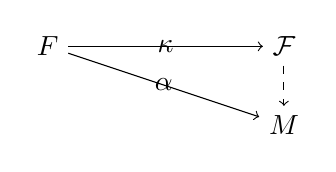
\begin{tikzpicture}
\label{comm:an-uni}
	\node (F) {$F$};
	\node (Fm) [right of=F, node distance=3cm] {$\mathcal F$};
	\node (M) [below of=Fm] {$M$};
	\draw [->] (F) to node {$\kappa$} (Fm);
	\draw [->] (F) to node [swap] {$\alpha$} (M);
	\draw [->, dashed] (Fm) to node [swap] {} (M);
\end{tikzpicture}


Явная формула для аналитического функтора. Для доказательства см (TODO)
\begin{equation}
\label{eq:an}
	\mathcal F = \sum\limits_n F[n] \times A^n / S_n
\end{equation}

Хочется построить аналог аналитического функтора для h-species

\begin{tikzpicture}
\label{comm:h-an}
	\node (B) {$HB$};
	\node (S1) [below of=B] {$HSet$};
	\node (S2) [right of=B, node distance=3cm] {$HSet$};
	\draw [right hook->] (B) to node [swap] {$i$} (S1);
	\draw [->] (B) to node {$F$} (S2);
	\draw [->] (S1) to node [swap] {$\mathcal F$} (S2);
\end{tikzpicture}

\begin{equation}
\label{eq:h-an}
	\mathcal F = \sum\limits_n F[\Bar n] \times A^{\Bar n} / B_n
\end{equation}
Где $A^{\Bar n}$ задает отображение, сохраняющее инволюцию. 

TODO:Здесь нужно добавить проверук универсальности картинки

\subsection{Декотигорификация аналитического функтора (Фробениусова
характеристика / Цикленный индекс)} 
\subsubsection{Случай обычных species}
Напомним ситуацию с обычными species. Надо устроить морфизм из моноидальной
категории (категории с тензорным произведением) в какую-нибудь алгебру функций. Мы вводим весовую
функцию таким образом что орбита раскрашенной структуры под действием $S_n$ имеет один и тот же вес.
После этого можно задать вопрос о коэфициенте при мономе, отвечающем весу. Это
будет число орбит с заданной весовой функцией. По Лемме Бернсайда это то же
самое, что и усредненное число неподвижных точек по всем элементам группы. Чтобы
раскрашенная структура была неподвижна под действием перестановки $\sigma$
нужно, чтобы во-первых она была неподвижна как не раскрашенная структура, а
во-вторых расскраска должна переходить в себя. В качестве
весовой функции выбираем моном возникающий в произведении переменных отвечающим
цветам. Например расскраске в которой 2 первых цвета и 1 второй
соответсвует моном $x_1^2x_2$. Тогда первое условие дает нам сомножитель
$\chi(\sigma)$, где характер это характер соответствующего перестановочного
представления с базисом из структур. Второе условие требует покраски каждого
цикла в один и тот же цвет. Итоговая формула называеться фробениусовой
характеристикой / цикленным индексом. Она считает количество неподвижных
раскрашенных структур в среднем. 

\begin{equation}
\label{eq:fr}
\mathcal Z_F = \sum_{\lambda \vdash n}\chi(\sigma_{\lambda})
\frac{\phi^{\lambda}}{z_{\lambda}}
\end{equation}

Где $\chi$ --- характер (перестановочного) представления заданного $F$, $\sigma$
--- перестановка цикленного типа $\lambda$, 
$\phi^{\lambda} = 
(x_1^{\lambda_1} + x_2^{\lambda_1} + x_3^{\lambda_1} + \dots)
(x_1^{\lambda_2} + x_2^{\lambda_2} + x_3^{\lambda_2} + \dots)
(x_1^{\lambda_3} + x_2^{\lambda_3} + x_3^{\lambda_3} + \dots)
\dots$,
 $z_\lambda$ --- индекс класса сопряженности $\sigma$.
Появляется она из следующих соображений: в числителе стоит симметрическая
функция считающая все неподвижные раскраски. Цвета это $x_1, x_2, x_3, \dots$

\subsubsection{Случай h-species}
Попробуем построить аналогичную конструкцию для h-species.
Прежде всего отметим, что расскраска, элемент $A^{\Bar n}$, это отображение,
сохраняющее инволюцию. Значит элементы $n$ и $-n$ должны отображаться либо в
один и тот же элемент $A$ (который инволюцией переводиться в себя), либо в пару
элементов сопряженных инволюцией. Будем называть первый случай
\emph{моноцветом}, второй --- \emph{бицветом}.	

Допустим, что мы придумали весовую функцию, отправляющую каждую расскрашенную
структуру в моном и любая орбита отправляеться в один моном. Применив Лемму
Бернсайда переходим к подсчету неподвижных точек. Циклы в каждом элементе $H_n$
бывают двух типов:
длинные --- каждая грань входит в цикл вместе со своей противоположной гранью и
короткие --- пара граней лежит в симметричных, различных циклах. Пусть
$\lambda^1$ --- цикленный тип коротких перестановок, $\lambda^2$ --- цикленный
тип длинных перестановок. Утверждение: неподвижные
раскрашенные структуры, это в точности те у которых длинный цикл соответсвует
моноцвету, а пара симметричных коротких может быть покрашена либо в моноцвет, либо в бицвет.

Это можно выразить такой формулой:
\begin{equation}
\label{eq:h-fr}
\sum_{\lambda^1 + \lambda^2 \vdash n}\chi(\sigma_{\lambda^1 \lambda^2})
\frac{\phi_{x, y}^{\lambda^1} \phi_{x}^{\lambda^2}}{z_{\lambda^1 \lambda^2}}
\end{equation}

Здесь нижний индекс $\phi$ означает переменные по которым берется степенная
сумма. Например $\phi_{x, y}^2 = 
(x_1^2 + x_2^2 + x_3^2 + \dots + y_1^2 + y_2^2 + y_3^2 + \dots)
$. Переменные $x_i$ перечисляют моноцвета, $y_i$ --- бицвета.

TODO:Здесь еще можно сказать что-то про инволюцию на этих функциях, поскольку мы
все--таки декатегорифицировали не предпучки, а чуть более сложную штуку ---
пучки с инволюцией.
